\documentclass[12pt]{beamer}

\usepackage{beamerthemesplit}


\usepackage{beamerthemesplit}

\usepackage{beamerStatisticsTAMU} 

\logo{\includegraphics[height=1.5cm]{STAT_Horz-Aggie-Maroon.pdf}\vspace{220pt}}


\usepackage{amsmath}
\usepackage{amssymb}
\usepackage{verbatim}
\usepackage{bibentry}
%\usepackage{biblatex}
%\usepackage{natbib}
\newcommand{\argmin}[1]{\underset{#1}{\operatorname{argmin}}\text{ }}
\newcommand{\argmax}[1]{\underset{#1}{\operatorname{argmax}}\text{ }}
\usepackage{bbm}
\usepackage{bm}


\newcommand{\Var}{\text{Var }}
\newcommand{\Cov}{\text{Cov }}
\newcommand{\E}{\mathbb{E}}
\newcommand{\ind}{\mathbbm{1}}
\newcommand{\V}[1]{{\bm{\mathbf{\MakeLowercase{#1}}}}} % vector
\newcommand{\M}[1]{{\bm{\mathbf{\MakeUppercase{#1}}}}} % matrix
\newcommand{\todo}[1]{{\color{red}TODO: #1}}


\usepackage[absolute,overlay]{textpos}

\newcommand{\att}[1]{\begin{textblock*}{12cm}(0.5cm,9cm) % {block width} (coords)
    {\tiny Source: #1}
\end{textblock*}}


\newcommand{\foot}[1]{\begin{textblock*}{12cm}(0.5cm,9cm) % {block width} (coords)
    {\tiny #1}
\end{textblock*}}




\newtheorem{assumptions}{Assumptions}

\setbeamertemplate{headline}[default]
\setbeamertemplate{footline}[page number]
\setbeamertemplate{navigation symbols}{}
\setbeamertemplate{bibliography item}[text]

\title{RR Lyrae Model and Feature Updates}
%%\author{James Long}
%%\institute{UC Berkeley}
\date{\today}
\begin{document}

\frame{\titlepage}


\AtBeginSection[]
{
  \begin{frame}<beamer>
    %\frametitle{Outline}
    \tableofcontents[currentsection,currentsubsection]
  \end{frame}
}



\section{Template / Code Improvements}

\begin{frame}{Old Template Shapes: Sloan Filters}
  \begin{center}
    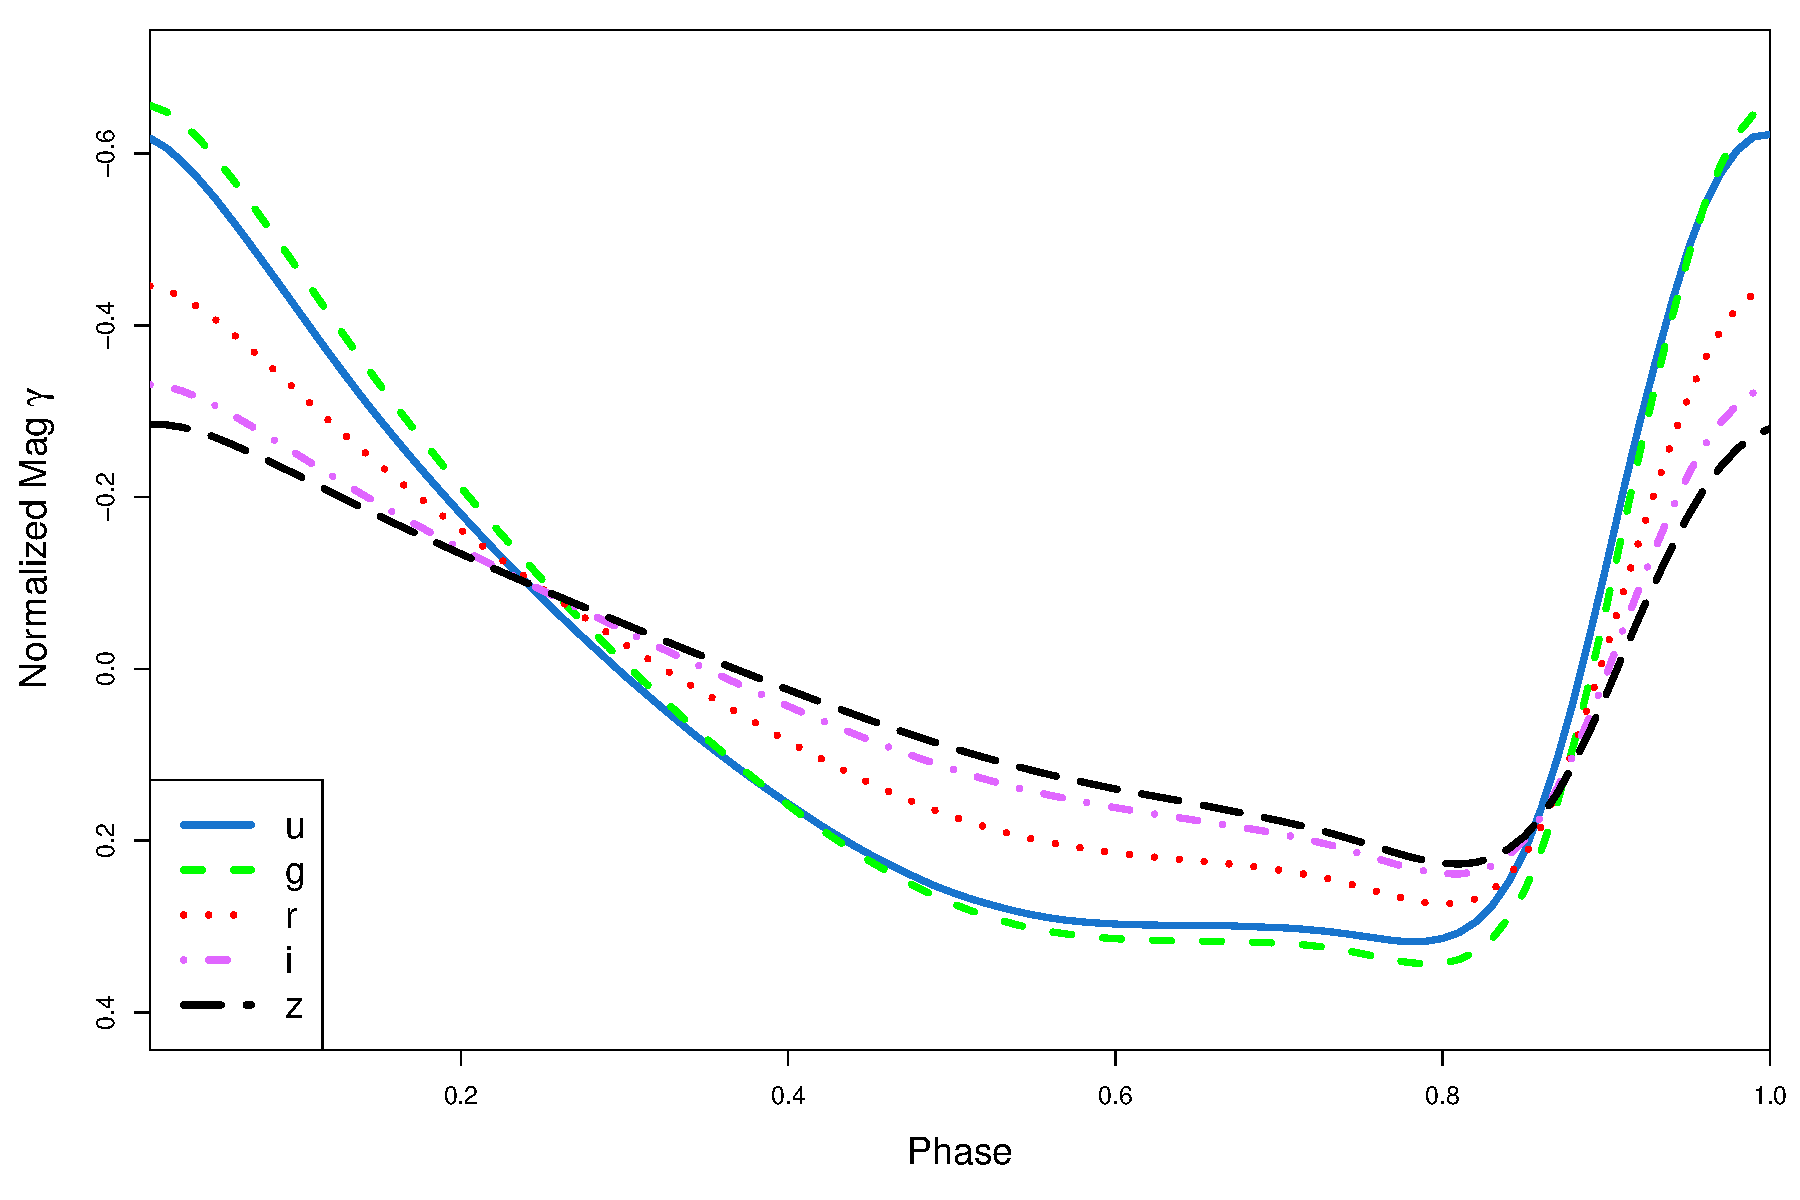
\includegraphics[scale=0.35]{figs/sdss_templates_old.pdf}
  \end{center}
\end{frame}


\begin{frame}{New Template Shapes: Sloan Filters}
  \begin{center}
    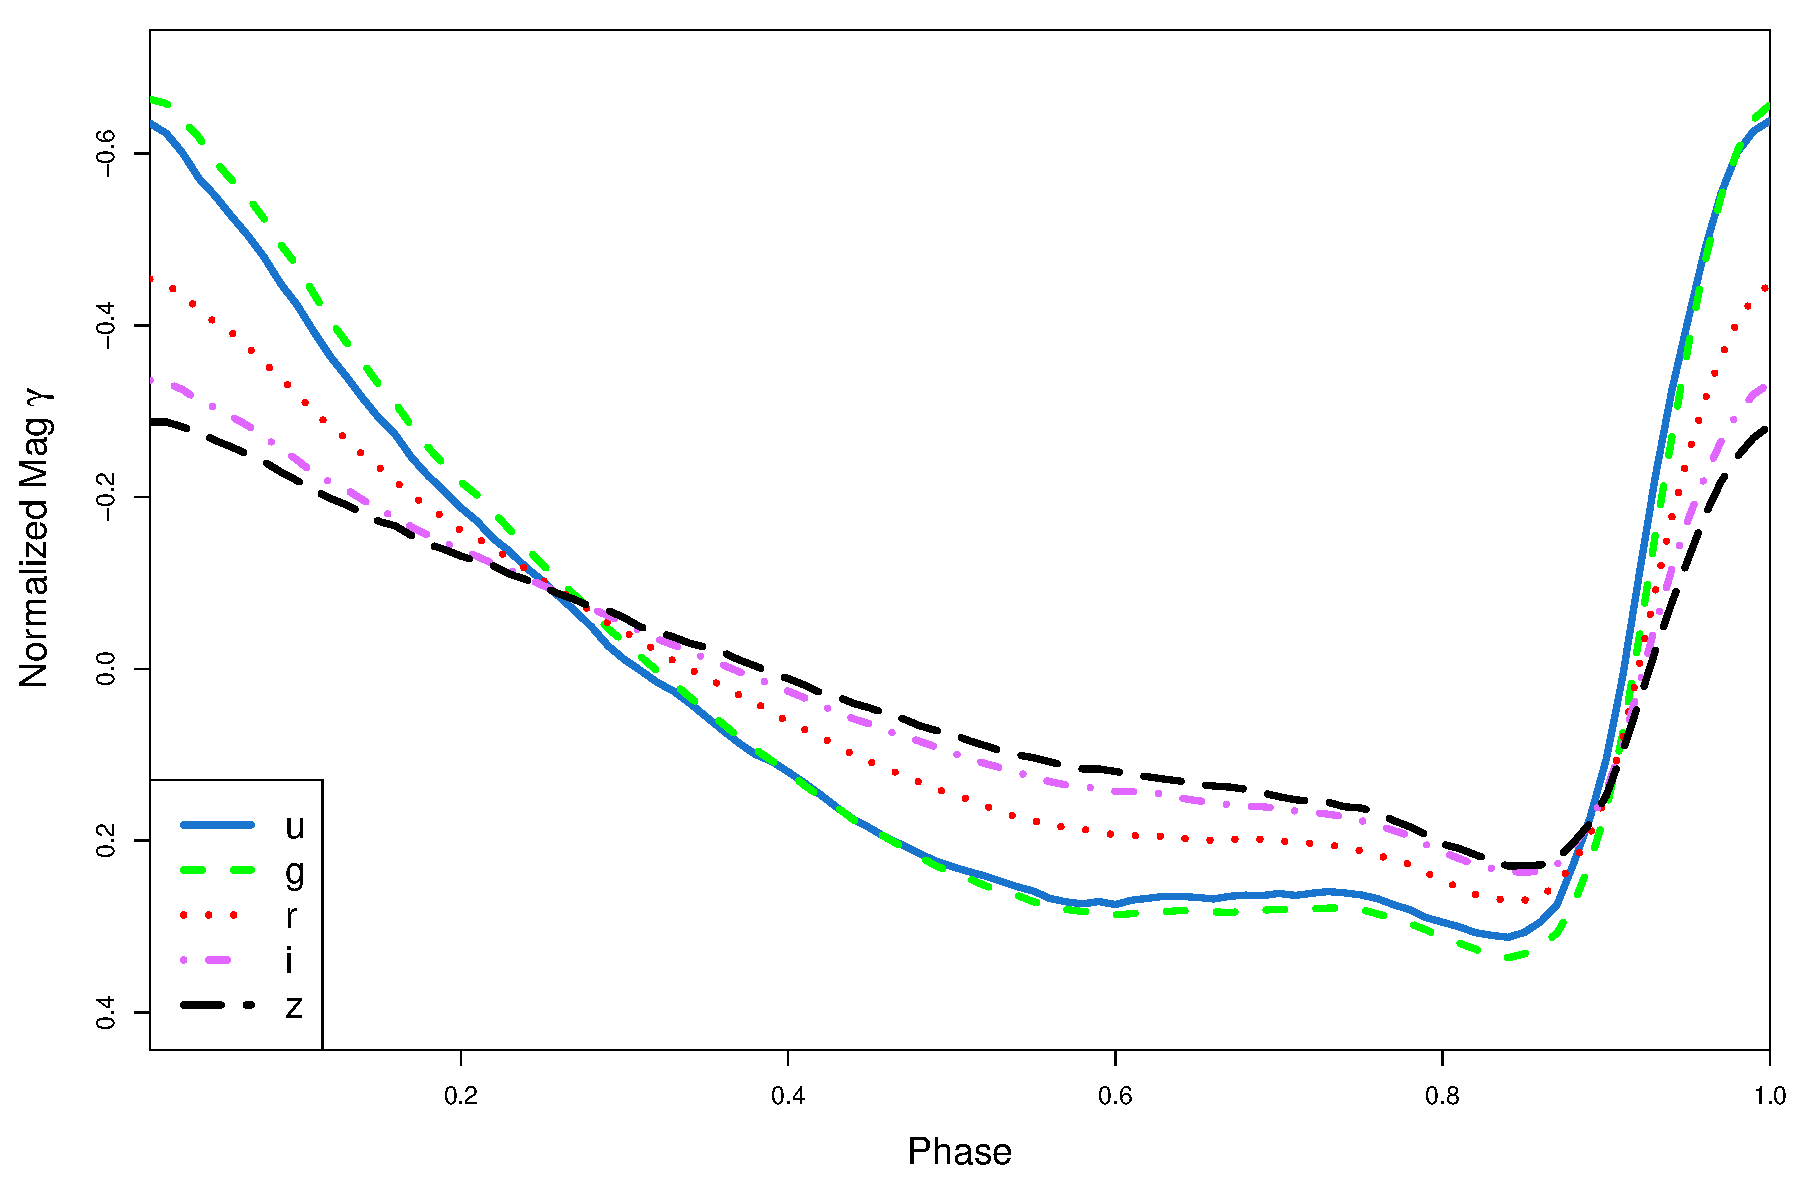
\includegraphics[scale=0.35]{figs/sdss_templates.pdf}
  \end{center}
\end{frame}

%% \begin{frame}{Template Shapes: DES Filters}
%%   \begin{center}
%%     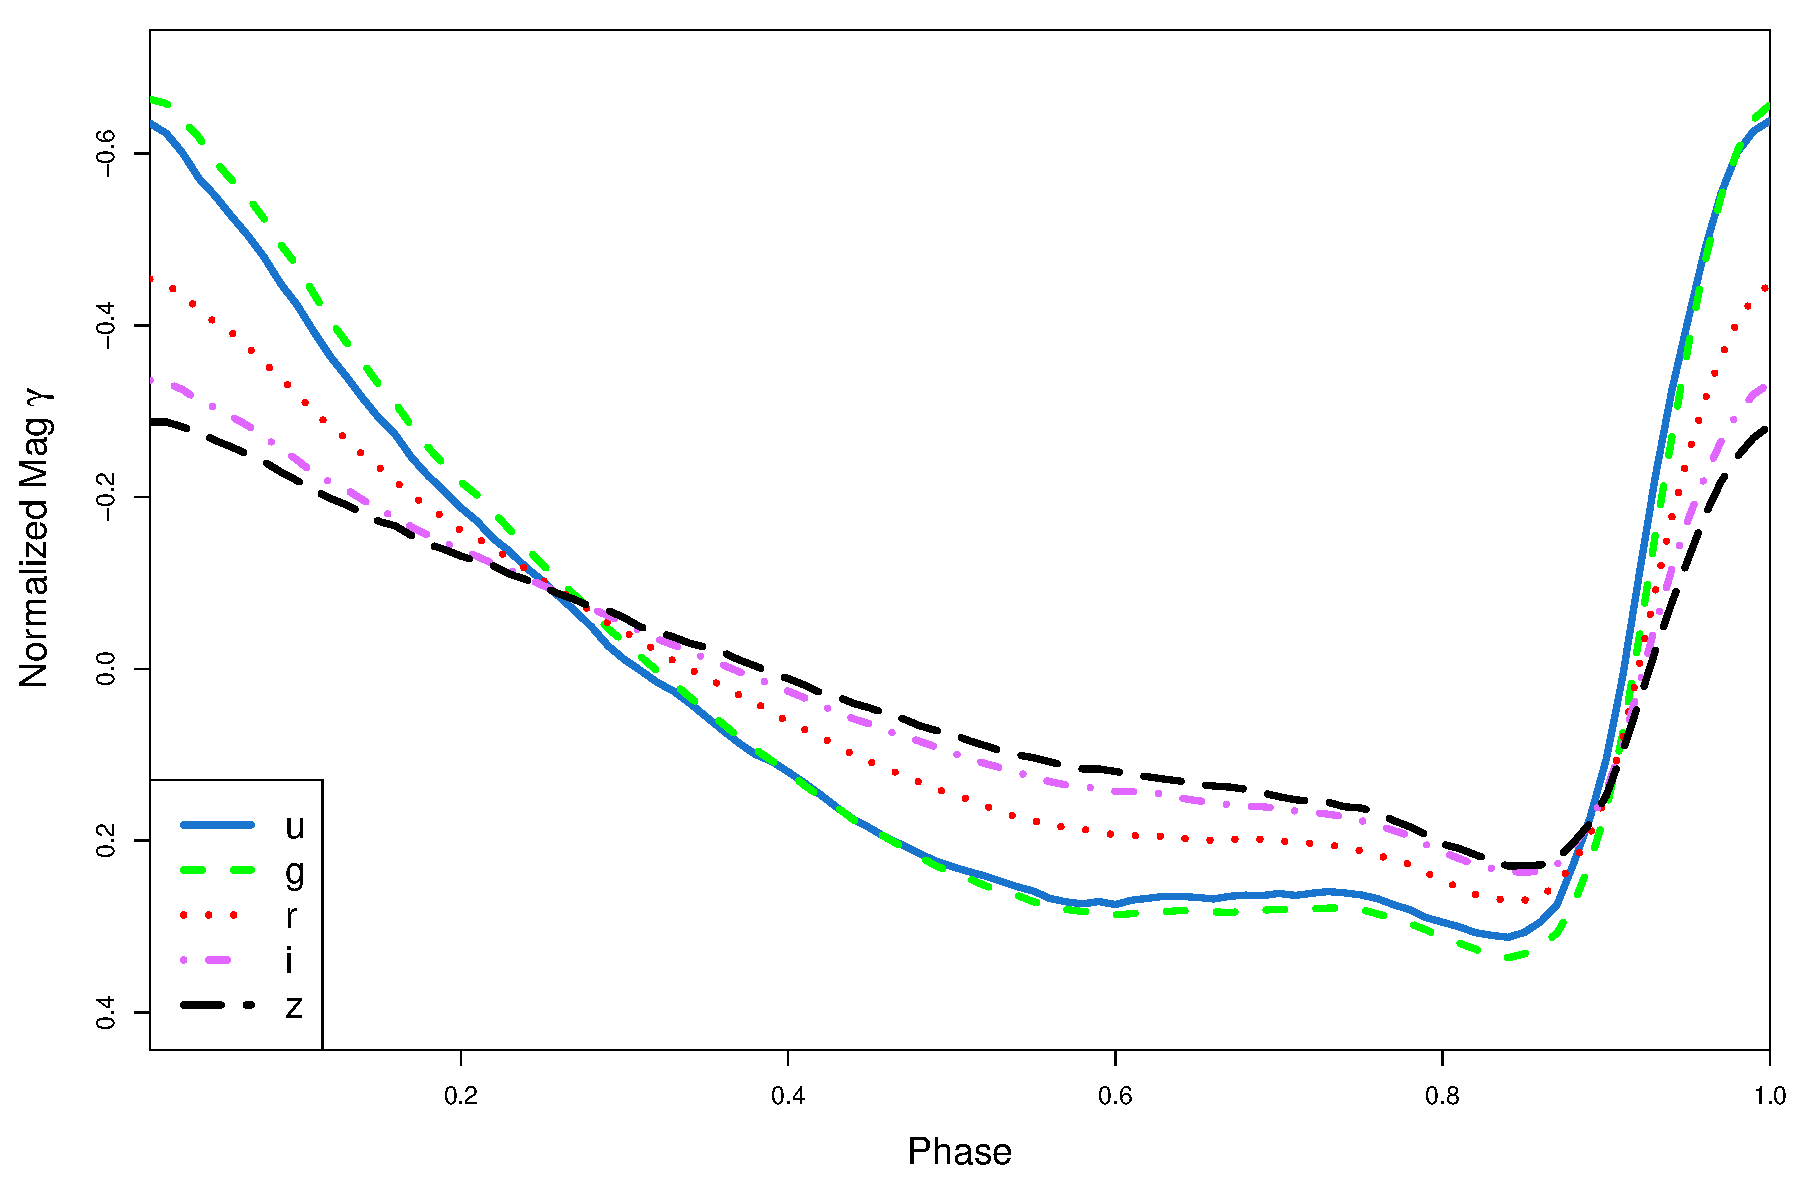
\includegraphics[scale=0.3]{figs/sdss_templates.pdf}
%%   \end{center}
%% \end{frame}



%% \begin{frame}{Summary}
%%   \begin{itemize}
%%   \item old template construction code ``oversmoothed'' light curves
%%   \item local minimum and maximum were biased towards $0$
%%   \item model error\\
%%     \begin{itemize}
%%     \item old templates: $0.02$ mags TODO: check this
%%     \item new templates:
%%     \end{itemize}
%%   \end{itemize}    

%%   \end{frame}


%% \begin{frame}{Model}
%%   \underline{Model with Dust:}
%%   Let $m_{ibj}$ be the magnitude measurement at time $t_{ibj}$ in band $j$. Then
%%   \begin{equation*}
%%     m_{ibj} = \mu + M_b + E[B-V]R_b + a\gamma_b(\omega t_{ibj} + \phi) + \epsilon_{ibj}
%%   \end{equation*}
  
%%   \underline{Model without Dust:}
%%   Let
%%   \begin{equation*}
%%     m_{ibj}' = m_{ibj} - E[B-V]R_b
%%   \end{equation*}
%%   be dust correct mag at time $t_{ibj}$. Then
%%   \begin{equation*}
%%     m_{ibj} = \mu + M_b + a\gamma_b(\omega t_{ibj} + \phi) + \epsilon_{ibj}
%%   \end{equation*}


%%   \begin{itemize}
%%   \item Old code always fit dust
%%   \item Dust corrected lightcurves input into old code would return dust $\approx 0$ (hopefully)
%%   \item But if we know dust, can get better fits for other parameters by not fitting it.
%%   \end{itemize}
  
%% \end{frame}


\begin{frame}{Dust and Photometric Errors}
  \begin{itemize}
    \item Dust
  \begin{itemize}
  \item Old code always fit dust
  \item Dust corrected lightcurves input into old code would return dust $\approx 0$ (hopefully)
  \item But if we know dust, can get better fits for other parameters by not fitting it.
  \item New code optionally fits dust.
  \end{itemize}
\item Photometric error
  \begin{itemize}
  \item Photometric errors not used in old code fitting.
  \item Using photometric errors but not model error is dangerous (overweights obs with low photometric error)
  \item New code (optionally) uses model and photometric uncertainty
  \end{itemize}
  \end{itemize}
  \end{frame}


\begin{frame}[fragile]{FitTemplate R Function}

  \begin{center}
    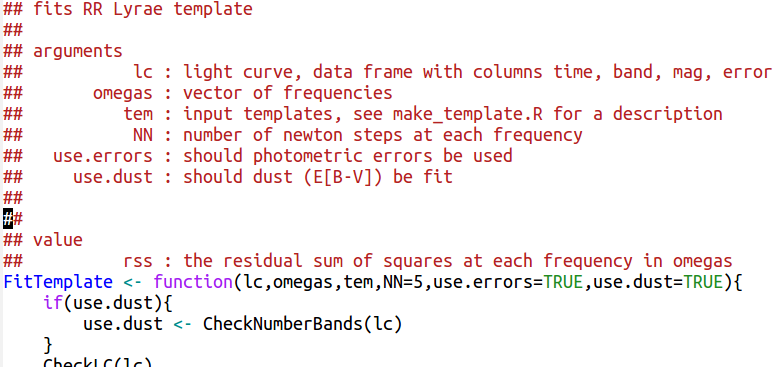
\includegraphics[scale=0.2]{figs/FitTemplate.png}
  \end{center}

  \underline{Call from Python, Fitting for Dust:}

 % \vspace{-.1in}

\begin{verbatim}
  rss=FitTemplate(lc,omegas,r.tem)
\end{verbatim}

%\vspace{-.1in}

  \underline{Call from Python, Not Fitting for Dust:}  \\
  
\begin{verbatim}
NN = IntVector(np.array([5],dtype='int'))
use_errors = BoolVector(np.array([True],dtype='bool'))
use_dust = BoolVector(np.array([False],dtype='bool'))
rss=FitTemplate(lc,omegas,r.tem,NN,use_errors,use_dust)
\end{verbatim}

  
\vspace{.1in}
  
See \texttt{template.py} file for examples.
  
\end{frame}


\section{Alias Detection Feature}

\begin{frame}{Aliasing with SDSS Data}

  \begin{center}
  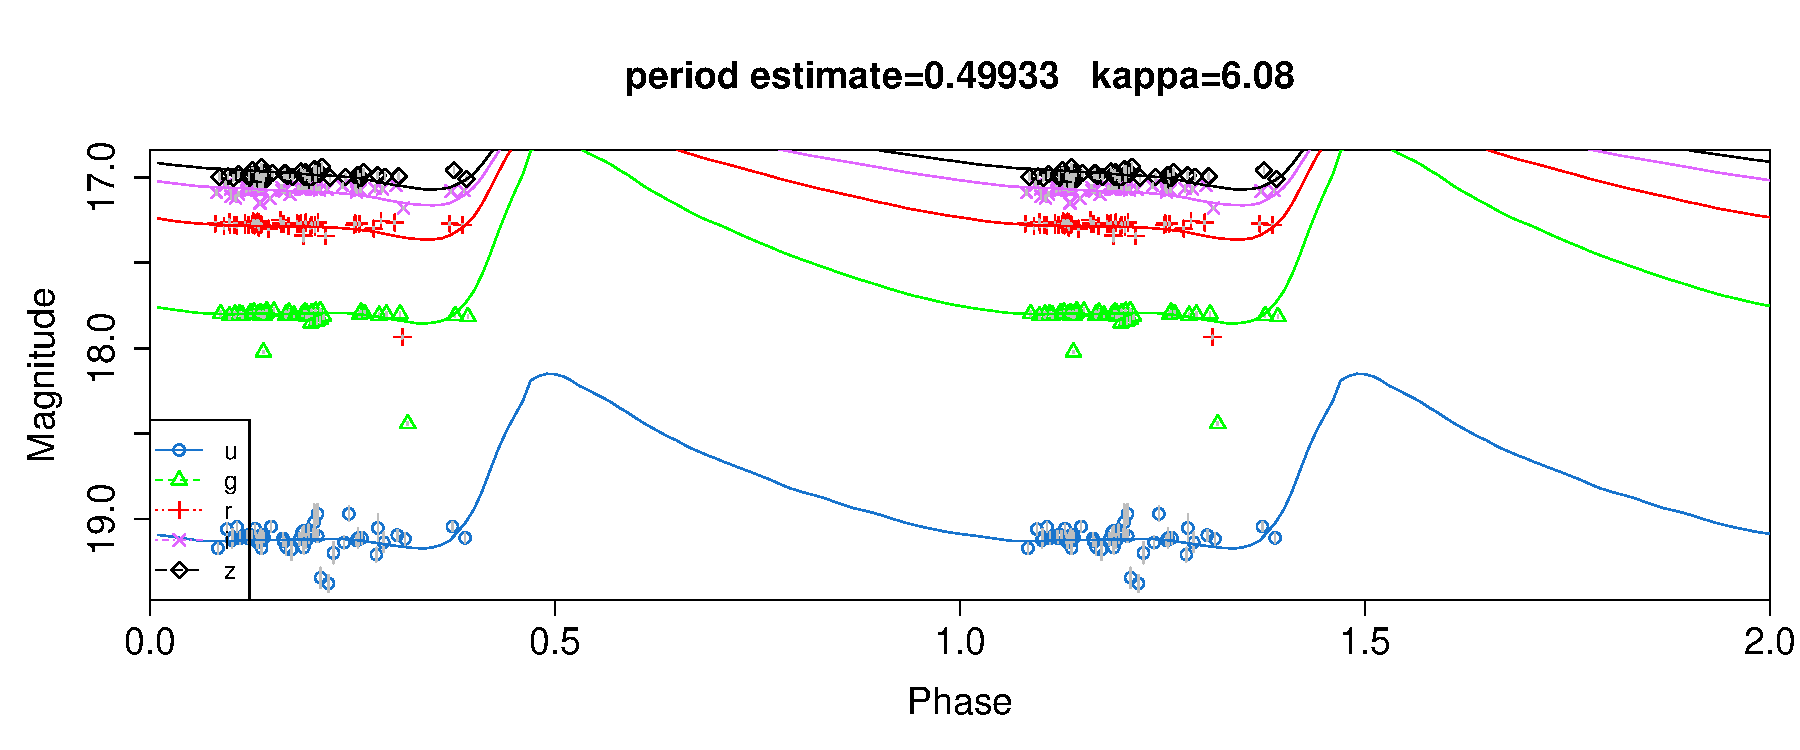
\includegraphics[scale=0.3]{figs/alias_not_rr.pdf}\\
  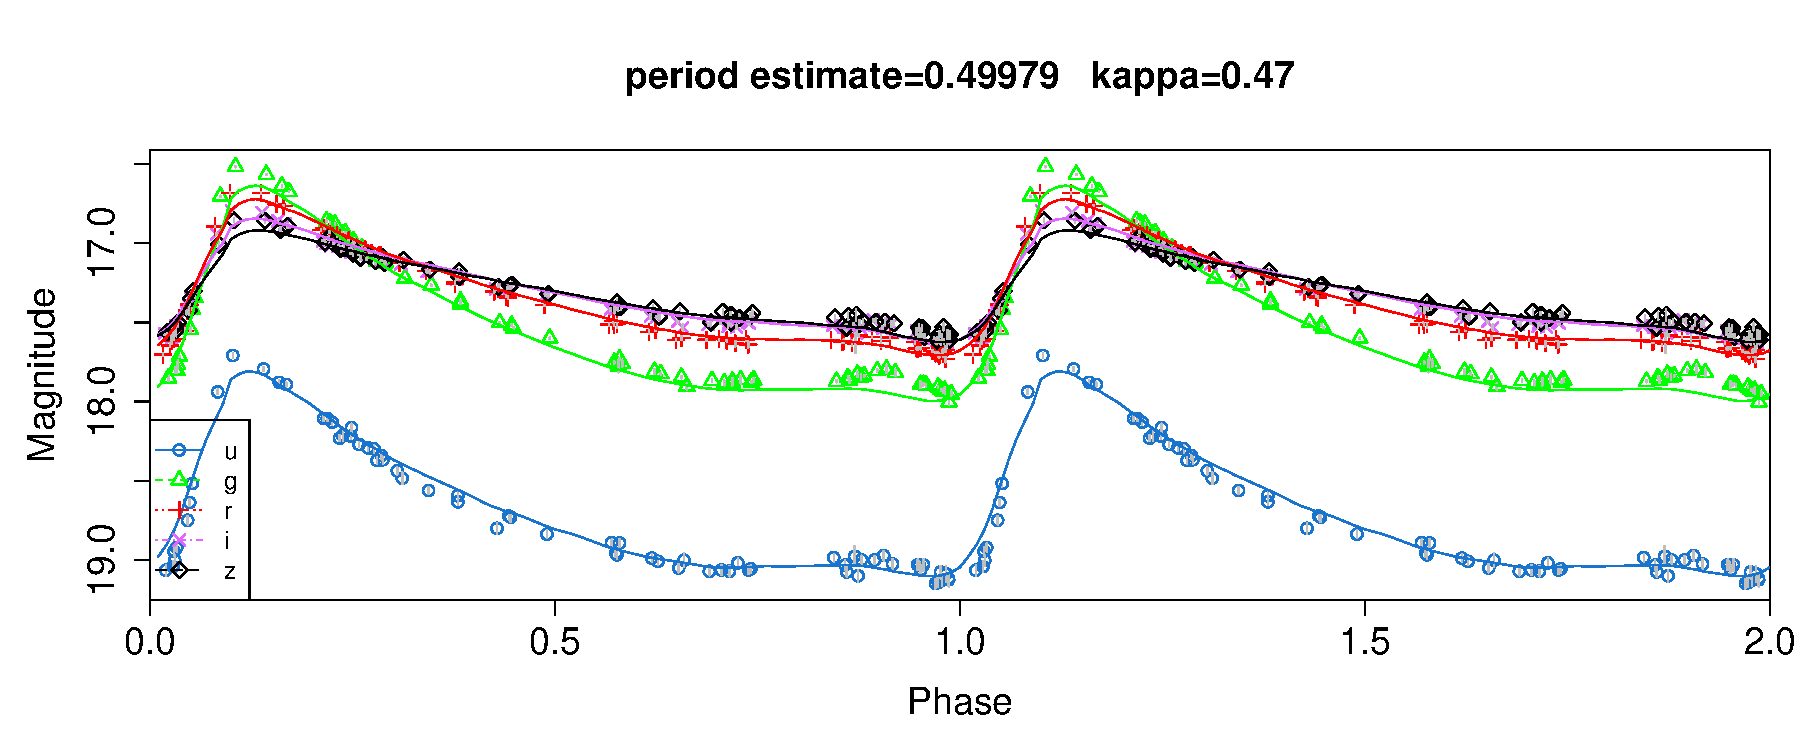
\includegraphics[scale=0.3]{figs/alias_rr_rr.pdf}
  \end{center}
  
\end{frame}




\begin{frame}[fragile]{Feature to Detect Aliasing}
Measure ``spread'' of epochs in phase space:
    \begin{itemize}
    \item \textbf{low spread:} eliminate light curve
    \item \textbf{high spread:} keep (use other parameter to classify)
    \item $\kappa$ parameter from fisher-von mises distribution measures spread
  \end{itemize}

\vspace{.1in}
    
\underline{Python code for computing $\kappa$}:
\begin{verbatim}
## arguments
##        phi : vector of phases on [0,1)
## value
##        1-step mle of kappa from
##        fisher von mises dist on unit circle
def kappa(phi):
    x = np.sum(np.cos(2*np.pi*phi))
    y = np.sum(np.sin(2*np.pi*phi))
    rbar = np.sqrt(x*x + y*y) / np.size(phi)
    return (rbar*(2.-rbar**2)) / (1.-rbar**2)
\end{verbatim}

\end{frame}


%% \begin{frame}[fragile]{Computing $\kappa$}

%% \begin{verbatim}
%% ## arguments
%% ##        phi : vector of phases on [0,1)
%% ## value
%% ##        1-step mle of kappa from
%% ##        fisher von mises dist on unit circle
%% def kappa(phi):
%%     x = np.sum(np.cos(2*np.pi*phi))
%%     y = np.sum(np.sin(2*np.pi*phi))
%%     rbar = np.sqrt(x*x + y*y) / np.size(phi)
%%     return (rbar*(2.-rbar**2)) / (1.-rbar**2)
%% \end{verbatim}
  
  
%% \end{frame}



\begin{frame}{Aliasing with SDSS Data}

  \begin{center}
  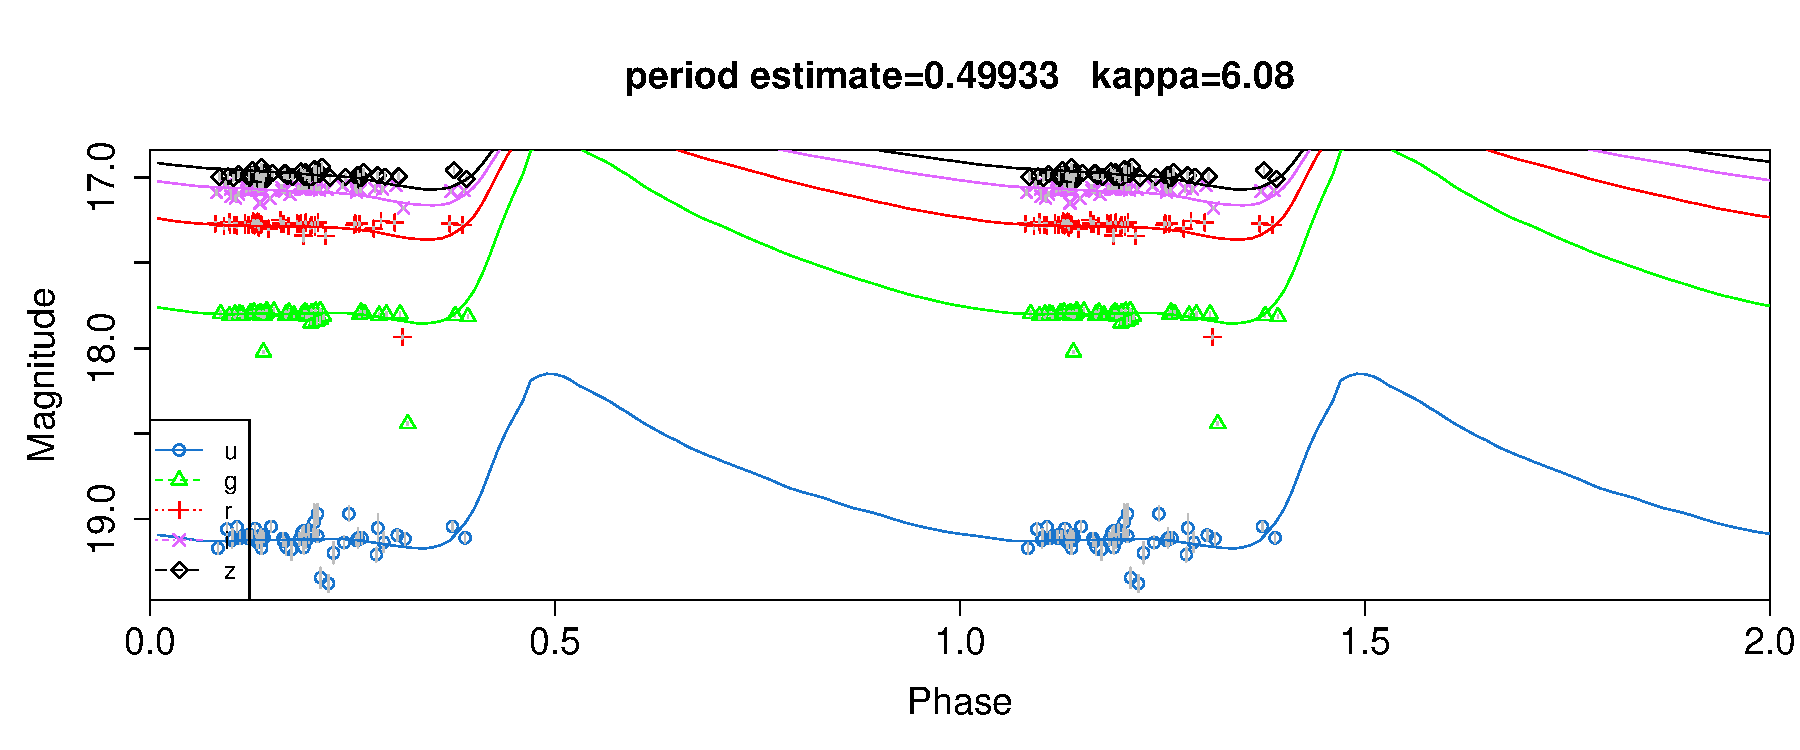
\includegraphics[scale=0.3]{figs/alias_not_rr.pdf}\\
  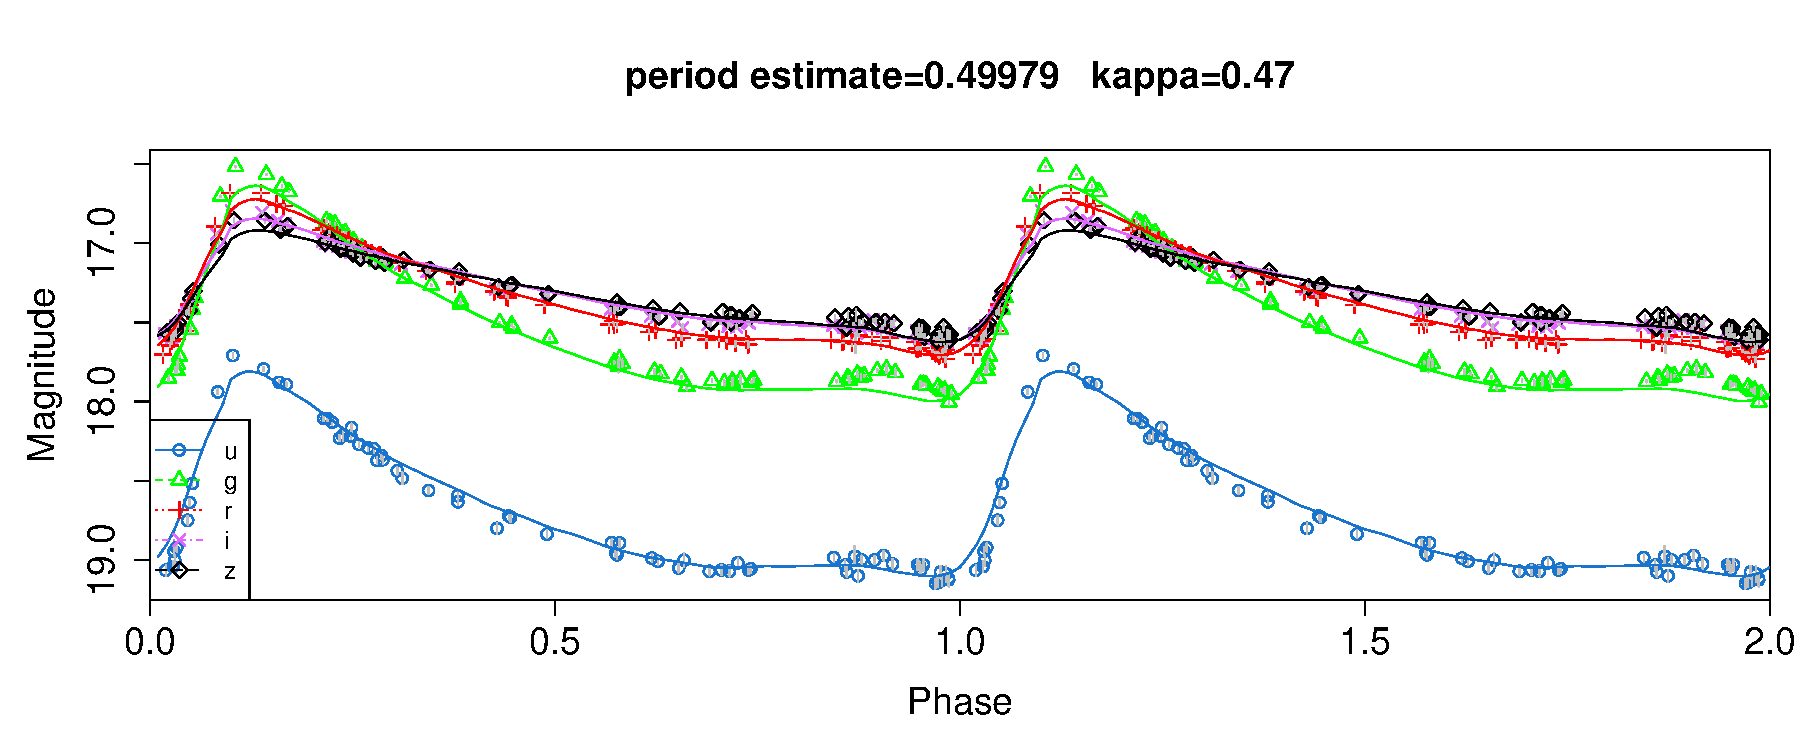
\includegraphics[scale=0.3]{figs/alias_rr_rr.pdf}
  \end{center}
  
\end{frame}




\begin{frame}{$\kappa$ versus Period Estimate SDSS}

  \begin{center}
  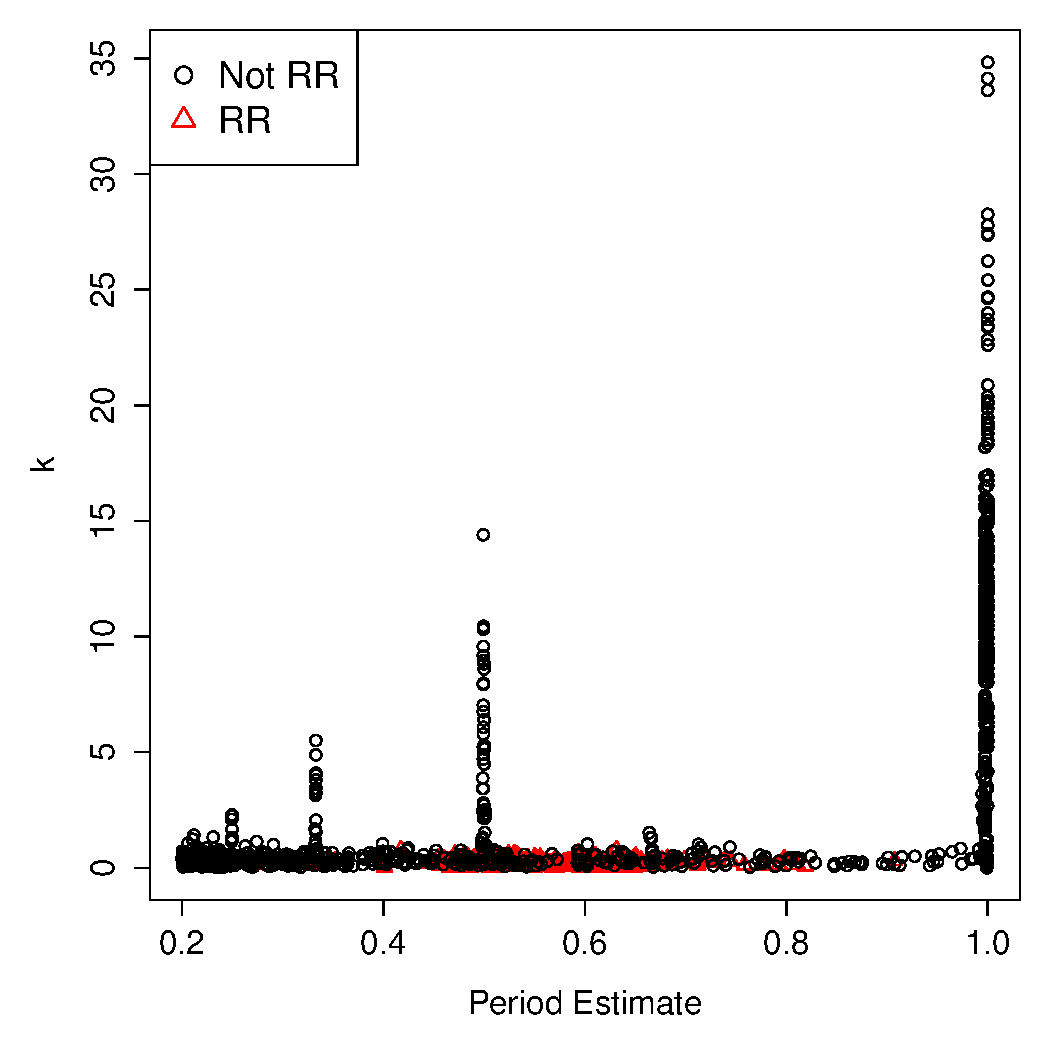
\includegraphics[scale=0.45]{figs/kappa_period_sdss.pdf}
  \end{center}
  
\end{frame}


\section{Suggestions for Using the Model}

\begin{frame}{Suggestion for Classification Pipeline}
  \begin{itemize}
    \item possible pipeline
  \begin{enumerate}
  \item remove obvious non RRL based on variability, colors
  \item fit model to all remaining sources
  \item remove all sources with $\kappa > c$
  \item remove all sources with $E[B-V]$ outside $[-\epsilon,d]$ 
  \item identify RRL based on (amp,period,RSS) cuts
  \end{enumerate}
  \item precise cuts can be chosen using DES light curves cross matched with Sloan in Stripe 82
  \item somewhat skeptical of using random forest for this application, mainly because of training / test set differences
  \end{itemize}
  


\end{frame}


\begin{frame}{Sanity Checks / To Dos (for Katelyn)}

\textbf{Warning:} Code may have bugs. Please do sanity checks:
  
  \begin{itemize}
  \item \textbf{sanity check 1:} model dust estimates close to dust maps?
  \item \textbf{sanity check 2:} perturb a few magnitudes, check updated model fits with use.errors=TRUE and use.errors=FALSE
  \item \textbf{sanity check 3:} better results than before
  \item \textbf{sanity check X:} lots of other possibilities
  \end{itemize}

\vspace{.2in}
  
\textbf{Important to do:} determine whether sesar distances or model distances are more accurate, use better method
\end{frame}

\end{document}


